\pagestyle{fancy}
\section{Results}
% AUTO-GENERATED by analysis/generate-results-tex.ts — do not edit by hand.
% Regenerate: cd analysis && bun run gen-tex

\providecommand{\GenNTotal}{0}
\providecommand{\GenNValid}{19}
\providecommand{\GenDemoAge}{19 (5); 20 (1); 21 (3); 22 (6); 23 (3); 24 (1)}
\providecommand{\GenDemoWebMdn}{6.0}
\providecommand{\GenDemoWebIqr}{6.0--7.0}
\providecommand{\GenDemoAiMdn}{6.0}
\providecommand{\GenDemoAiIqr}{5.0--7.0}
\providecommand{\GenCounterBaselineFirstN}{11}
\providecommand{\GenCounterBaselineFirstPct}{58}
\providecommand{\GenCounterEphemeralFirstN}{8}
\providecommand{\GenCounterEphemeralFirstPct}{42}
\providecommand{\GenCompNBaseline}{11}
\providecommand{\GenCompNEphemeral}{13}
\providecommand{\GenCompPctBaseline}{57.9}
\providecommand{\GenCompPctEphemeral}{68.4}
\providecommand{\GenCompMcNemarP}{0.500}
\providecommand{\GenTimeBaselineMdn}{35.7}
\providecommand{\GenTimeBaselineIqr}{16.4--73.4}
\providecommand{\GenTimeEphemeralMdn}{56.9}
\providecommand{\GenTimeEphemeralIqr}{23.0--85.1}
\providecommand{\GenTimeWilcoxonResult}{did not yield a statistically significant difference}
\providecommand{\GenTimeW}{80}
\providecommand{\GenTimeP}{0.568}
\providecommand{\GenTimeR}{0.158}
\providecommand{\GenIntBaselineMdn}{3.0}
\providecommand{\GenIntBaselineIqr}{1.0--4.0}
\providecommand{\GenIntEphemeralMdn}{11.0}
\providecommand{\GenIntEphemeralIqr}{5.0--13.0}
\providecommand{\GenIntWilcoxonResult}{yielded a statistically significant difference}
\providecommand{\GenIntW}{0}
\providecommand{\GenIntP}{\textless 0.001}
\providecommand{\GenIntR}{1.000}
\providecommand{\GenLikertHelpfulnessBaselineMdn}{5.0}
\providecommand{\GenLikertHelpfulnessBaselineIqr}{3.0--6.0}
\providecommand{\GenLikertHelpfulnessEphemeralMdn}{6.0}
\providecommand{\GenLikertHelpfulnessEphemeralIqr}{5.0--6.0}
\providecommand{\GenLikertHelpfulnessP}{0.048}
\providecommand{\GenLikertIntrusivenessBaselineMdn}{3.0}
\providecommand{\GenLikertIntrusivenessBaselineIqr}{2.0--5.0}
\providecommand{\GenLikertIntrusivenessEphemeralMdn}{5.0}
\providecommand{\GenLikertIntrusivenessEphemeralIqr}{4.0--6.0}
\providecommand{\GenLikertIntrusivenessP}{0.021}
\providecommand{\GenLikertControlBaselineMdn}{6.0}
\providecommand{\GenLikertControlBaselineIqr}{4.5--7.0}
\providecommand{\GenLikertControlEphemeralMdn}{6.0}
\providecommand{\GenLikertControlEphemeralIqr}{4.5--6.0}
\providecommand{\GenLikertControlP}{0.635}
\providecommand{\GenPrefOverallB}{4}
\providecommand{\GenPrefOverallE}{9}
\providecommand{\GenPrefOverallN}{6}
\providecommand{\GenPrefHelpB}{6}
\providecommand{\GenPrefHelpE}{10}
\providecommand{\GenPrefHelpN}{3}
\providecommand{\GenPrefIntrB}{1}
\providecommand{\GenPrefIntrE}{15}
\providecommand{\GenPrefIntrN}{3}
\providecommand{\GenPrefLifeB}{7}
\providecommand{\GenPrefLifeE}{8}
\providecommand{\GenPrefLifeN}{4}
\providecommand{\GenPrefOverallBinomialP}{0.267}
\providecommand{\GenEngNTriggered}{17}
\providecommand{\GenEngPctTriggered}{89.5}
\providecommand{\GenEngNUsed}{4}
\providecommand{\GenEngNDismissed}{17}
\providecommand{\GenEngNIgnored}{2}
\providecommand{\GenEngNExpanded}{3}
\providecommand{\GenEngTotalGen}{37}
\providecommand{\GenEngFallbackCount}{37}
\providecommand{\GenEngFallbackPct}{100.0}
\providecommand{\GenSumCompPctB}{57.9}
\providecommand{\GenSumCompPctE}{68.4}
\providecommand{\GenSumMcNemarP}{0.500}
\providecommand{\GenSumTimeBMdn}{35.7}
\providecommand{\GenSumTimeEMdn}{56.9}
\providecommand{\GenSumTimeP}{0.568}
\providecommand{\GenSumIntBMdn}{3.0}
\providecommand{\GenSumIntEMdn}{11.0}
\providecommand{\GenSumIntP}{\textless 0.001}
\providecommand{\GenSumHelpBMdn}{5.0}
\providecommand{\GenSumHelpEMdn}{6.0}
\providecommand{\GenSumHelpP}{0.048}
\providecommand{\GenSumIntrBMdn}{3.0}
\providecommand{\GenSumIntrEMdn}{5.0}
\providecommand{\GenSumIntrP}{0.021}
\providecommand{\GenSumCtrlBMdn}{6.0}
\providecommand{\GenSumCtrlEMdn}{6.0}
\providecommand{\GenSumCtrlP}{0.635}
\providecommand{\GenSumPrefOverall}{4 chose baseline; 9 chose ephemeral; 6 no preference}
\providecommand{\GenSumPrefOverallP}{0.267}



% ============================================================================
% HOW TO USE THIS SECTION
% ============================================================================
% 1. From analysis/: `bun install` then `bun run analyse` to export CSVs, print
%    statistics, rebuild figure PDFs in graphics/, and regenerate
%    `sections/generated-result-values.tex` (see analysis/README.md).
%    Or run analysis/queries.sql in psql.
% 2. Numeric values in tables and prose come from \texttt{generated-result-values.tex}
%    (run \texttt{bun run gen-tex} after export, or use \texttt{bun run analyse}).
% 3. After export: `bun run figures` in analysis/ writes PDFs to graphics/.
%    Re-run figures whenever you refresh the CSVs.
% ============================================================================

This section reports the outcomes of the comparative user study. All measures follow the analysis plan described in the methodology: behavioural data was extracted from the experiment database, and self-reported ratings were collected through post-trial and post-study questionnaires administered within the same website. Unless stated otherwise, paired comparisons use the Wilcoxon signed-rank test, medians and interquartile ranges (IQR) are reported for continuous and ordinal measures, and statistical significance is assessed at $\alpha = .05$.

\subsection{Participants and Data Overview}

% SQL — participant overview:
% SELECT
%   count(*) AS total_participants,
%   count(*) FILTER (WHERE consented_at IS NOT NULL) AS consented,
%   count(*) FILTER (WHERE instruction_acknowledged_at IS NOT NULL) AS started
% FROM participants;
%
% SQL — completed participants (both trials done + final questionnaire):
% SELECT p.id, p.age_range, p.occupation,
%        p.web_app_familiarity, p.ai_tool_familiarity,
%        p.baseline_is_version_a
% FROM participants p
% WHERE (SELECT count(*) FROM trials t
%        WHERE t.participant_id = p.id AND t.completed = true) = 2
%   AND (SELECT count(DISTINCT question_key) FROM questionnaire_responses qr
%        WHERE qr.participant_id = p.id AND qr.trial_id IS NULL
%          AND qr.question_key IN ('final_preference','final_helpfulness',
%                                  'final_intrusiveness','final_real_life')) = 4;
%
% SQL — background demographics summary:
% WITH valid AS ( <the query above> )
% SELECT
%   age_range,
%   count(*) AS n,
%   round(avg(web_app_familiarity), 1) AS mean_web,
%   round(avg(ai_tool_familiarity), 1) AS mean_ai
% FROM valid
% GROUP BY age_range ORDER BY age_range;

A total of \GenNTotal{} participants accessed the study website. Of these, \GenNValid{} completed both task trials and the final questionnaire and are included in the analysis. The remaining participants were excluded because they did not finish both conditions or did not complete the post-study questions. Table~\ref{tab:demographics} summarises the background characteristics of the included sample.

\begin{table}[htbp]
    \centering
    \caption{Participant background characteristics ($n = \GenNValid$).}
    \label{tab:demographics}
    \begin{tabular}{@{}lc@{}}
        \toprule
        Characteristic & Summary \\
        \midrule
        Age range & \GenDemoAge{} \\
        Web application familiarity (1--7) & Mdn = \GenDemoWebMdn{}, IQR = \GenDemoWebIqr{} \\
        AI tool familiarity (1--7) & Mdn = \GenDemoAiMdn{}, IQR = \GenDemoAiIqr{} \\
        Condition order: baseline first & \GenCounterBaselineFirstN{} (\GenCounterBaselineFirstPct{}\%) \\
        Condition order: ephemeral first & \GenCounterEphemeralFirstN{} (\GenCounterEphemeralFirstPct{}\%) \\
        \bottomrule
    \end{tabular}
\end{table}

\subsection{Task Completion Rate}

% SQL — completion rate per condition:
% SELECT t.condition,
%        count(*) AS n,
%        count(*) FILTER (WHERE t.completed AND t.correct) AS completed_correct,
%        round(100.0 * count(*) FILTER (WHERE t.completed AND t.correct) / count(*), 1) AS pct
% FROM trials t
% JOIN ( <valid participants subquery> ) v ON v.id = t.participant_id
% GROUP BY t.condition;
%
% SQL — paired completion data for McNemar's test:
% SELECT
%   b.participant_id,
%   b.completed AND b.correct AS baseline_correct,
%   e.completed AND e.correct AS ephemeral_correct
% FROM trials b
% JOIN trials e ON e.participant_id = b.participant_id
%              AND e.condition = 'ephemeral'
% JOIN ( <valid participants subquery> ) v ON v.id = b.participant_id
% WHERE b.condition = 'baseline';

Task completion was defined as submitting the slide deck in the correct canonical order. In the baseline condition, \GenCompNBaseline{} of \GenNValid{} participants (\GenCompPctBaseline{}\%) completed the task correctly. In the ephemeral condition, \GenCompNEphemeral{} of \GenNValid{} (\GenCompPctEphemeral{}\%) completed correctly. McNemar's exact test comparing discordant pairs yielded $p = \GenCompMcNemarP{}$.

\thesistodo{If completion was near-universal in both conditions, note that the task may have been straightforward enough for ceiling effects to limit how informative this measure is.}

\subsection{Task Completion Time}

% SQL — completion time per condition:
% SELECT t.condition,
%        count(*) AS n,
%        round(avg(t.duration_ms / 1000.0), 1) AS mean_sec,
%        percentile_cont(0.5) WITHIN GROUP (ORDER BY t.duration_ms / 1000.0) AS median_sec,
%        percentile_cont(0.25) WITHIN GROUP (ORDER BY t.duration_ms / 1000.0) AS q1_sec,
%        percentile_cont(0.75) WITHIN GROUP (ORDER BY t.duration_ms / 1000.0) AS q3_sec
% FROM trials t
% JOIN ( <valid participants subquery> ) v ON v.id = t.participant_id
% WHERE t.completed = true
% GROUP BY t.condition;
%
% SQL — paired time data for Wilcoxon (export as CSV for R/Python):
% SELECT
%   b.participant_id,
%   b.duration_ms / 1000.0 AS baseline_sec,
%   e.duration_ms / 1000.0 AS ephemeral_sec
% FROM trials b
% JOIN trials e ON e.participant_id = b.participant_id
%              AND e.condition = 'ephemeral'
% JOIN ( <valid participants subquery> ) v ON v.id = b.participant_id
% WHERE b.condition = 'baseline'
%   AND b.completed = true AND e.completed = true;

Completion time was measured from the moment the participant started the trial to the moment they submitted their answer. Participants who completed the task in the baseline condition had a median time of \GenTimeBaselineMdn{}~seconds (IQR: \GenTimeBaselineIqr{}), compared to \GenTimeEphemeralMdn{}~seconds (IQR: \GenTimeEphemeralIqr{}) in the ephemeral condition. A Wilcoxon signed-rank test \GenTimeWilcoxonResult{} ($W = \GenTimeW$, $p = \GenTimeP$, $r = \GenTimeR$).

\begin{figure}[htbp]
    \centering
    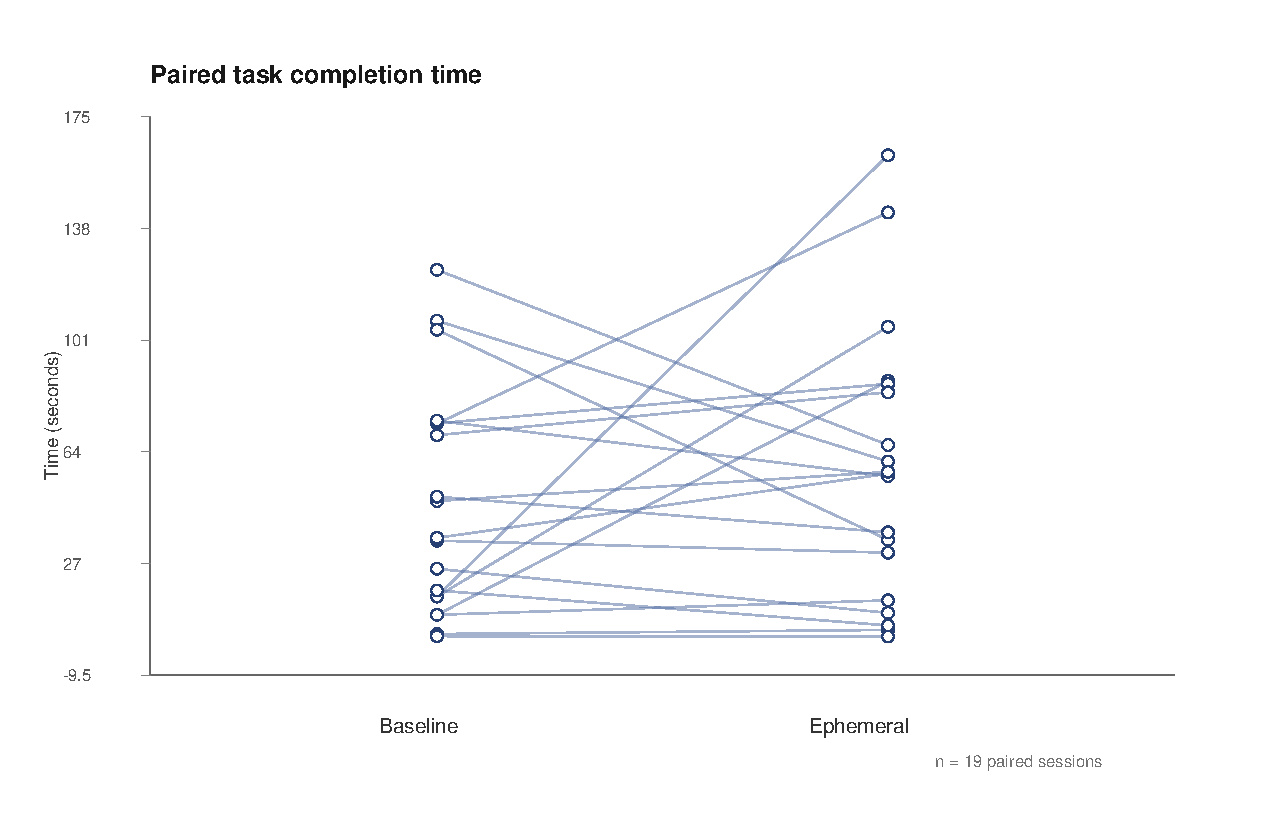
\includegraphics[width=0.65\textwidth]{graphics/results-completion-time.pdf}
    \caption{Paired comparison of task completion time (seconds) between the baseline and ephemeral conditions. Each line connects the same participant across conditions.}
    \label{fig:completion-time}
\end{figure}

\subsection{Interaction Count}

% SQL — interaction count per condition:
% SELECT t.condition,
%        count(*) AS n,
%        round(avg(t.interaction_count), 1) AS mean_interactions,
%        percentile_cont(0.5) WITHIN GROUP (ORDER BY t.interaction_count) AS median_interactions,
%        percentile_cont(0.25) WITHIN GROUP (ORDER BY t.interaction_count) AS q1,
%        percentile_cont(0.75) WITHIN GROUP (ORDER BY t.interaction_count) AS q3
% FROM trials t
% JOIN ( <valid participants subquery> ) v ON v.id = t.participant_id
% WHERE t.completed = true
% GROUP BY t.condition;
%
% SQL — paired interaction data for Wilcoxon (export as CSV):
% SELECT
%   b.participant_id,
%   b.interaction_count AS baseline_interactions,
%   e.interaction_count AS ephemeral_interactions
% FROM trials b
% JOIN trials e ON e.participant_id = b.participant_id
%              AND e.condition = 'ephemeral'
% JOIN ( <valid participants subquery> ) v ON v.id = b.participant_id
% WHERE b.condition = 'baseline'
%   AND b.completed = true AND e.completed = true;

The total number of logged interactions per trial was used as a proxy for task effort. The median interaction count in the baseline condition was \GenIntBaselineMdn{} (IQR: \GenIntBaselineIqr{}), compared to \GenIntEphemeralMdn{} (IQR: \GenIntEphemeralIqr{}) in the ephemeral condition. A Wilcoxon signed-rank test \GenIntWilcoxonResult{} ($W = \GenIntW$, $p = \GenIntP$, $r = \GenIntR$).

\thesistodo{Clarify that the ephemeral condition includes support-related interactions such as support shown and support dismissed. If the interaction count is higher, explain whether this reflects greater task effort or simply the extra steps introduced by the support layer.}

\begin{figure}[htbp]
    \centering
    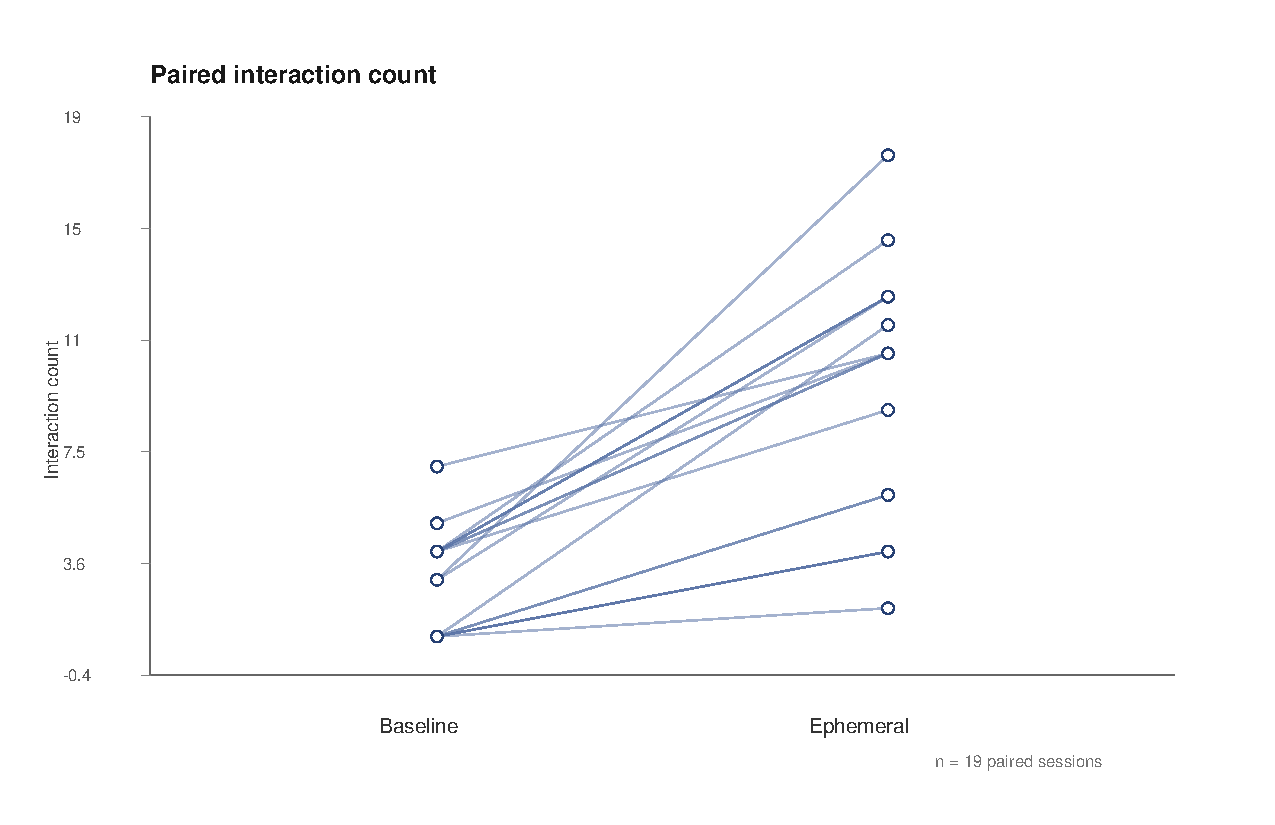
\includegraphics[width=0.65\textwidth]{graphics/results-interaction-count.pdf}
    \caption{Paired comparison of interaction count between the baseline and ephemeral conditions.}
    \label{fig:interaction-count}
\end{figure}

\subsection{Subjective Ratings}

% SQL — post-trial Likert ratings per condition:
% SELECT t.condition, qr.question_key,
%        count(*) AS n,
%        percentile_cont(0.5) WITHIN GROUP (ORDER BY qr.response_value::int) AS median_rating,
%        percentile_cont(0.25) WITHIN GROUP (ORDER BY qr.response_value::int) AS q1,
%        percentile_cont(0.75) WITHIN GROUP (ORDER BY qr.response_value::int) AS q3
% FROM questionnaire_responses qr
% JOIN trials t ON t.id = qr.trial_id
% JOIN ( <valid participants subquery> ) v ON v.id = qr.participant_id
% WHERE qr.question_key IN ('helpfulness', 'intrusiveness', 'control')
% GROUP BY t.condition, qr.question_key
% ORDER BY qr.question_key, t.condition;
%
% SQL — paired Likert data for Wilcoxon (export as CSV):
% SELECT
%   b_qr.participant_id,
%   b_qr.question_key,
%   b_qr.response_value::int AS baseline_rating,
%   e_qr.response_value::int AS ephemeral_rating
% FROM questionnaire_responses b_qr
% JOIN trials b_t ON b_t.id = b_qr.trial_id AND b_t.condition = 'baseline'
% JOIN trials e_t ON e_t.participant_id = b_t.participant_id
%                AND e_t.condition = 'ephemeral'
% JOIN questionnaire_responses e_qr ON e_qr.trial_id = e_t.id
%                                  AND e_qr.question_key = b_qr.question_key
% JOIN ( <valid participants subquery> ) v ON v.id = b_qr.participant_id
% WHERE b_qr.question_key IN ('helpfulness', 'intrusiveness', 'control');

After each trial, participants rated the interface on three dimensions using a seven-point Likert scale. Table~\ref{tab:likert} summarises the results.

\begin{table}[htbp]
    \centering
    \caption{Post-trial subjective ratings (7-point Likert scale, 1 = low, 7 = high).}
    \label{tab:likert}
    \begin{tabular}{@{}lccccc@{}}
        \toprule
        Measure & \multicolumn{2}{c}{Baseline} & \multicolumn{2}{c}{Ephemeral} & Wilcoxon \\
        \cmidrule(lr){2-3} \cmidrule(lr){4-5}
        & Mdn & IQR & Mdn & IQR & $p$ \\
        \midrule
        Helpfulness & \GenLikertHelpfulnessBaselineMdn{} & \GenLikertHelpfulnessBaselineIqr{} & \GenLikertHelpfulnessEphemeralMdn{} & \GenLikertHelpfulnessEphemeralIqr{} & \GenLikertHelpfulnessP{} \\
        Intrusiveness & \GenLikertIntrusivenessBaselineMdn{} & \GenLikertIntrusivenessBaselineIqr{} & \GenLikertIntrusivenessEphemeralMdn{} & \GenLikertIntrusivenessEphemeralIqr{} & \GenLikertIntrusivenessP{} \\
        Perceived control & \GenLikertControlBaselineMdn{} & \GenLikertControlBaselineIqr{} & \GenLikertControlEphemeralMdn{} & \GenLikertControlEphemeralIqr{} & \GenLikertControlP{} \\
        \bottomrule
    \end{tabular}
\end{table}

\thesistodo{Add one short paragraph per measure interpreting direction and significance. Cover whether the ephemeral condition was rated as more helpful, whether it felt more intrusive, and whether perceived control remained stable or changed.}

\begin{figure}[htbp]
    \centering
    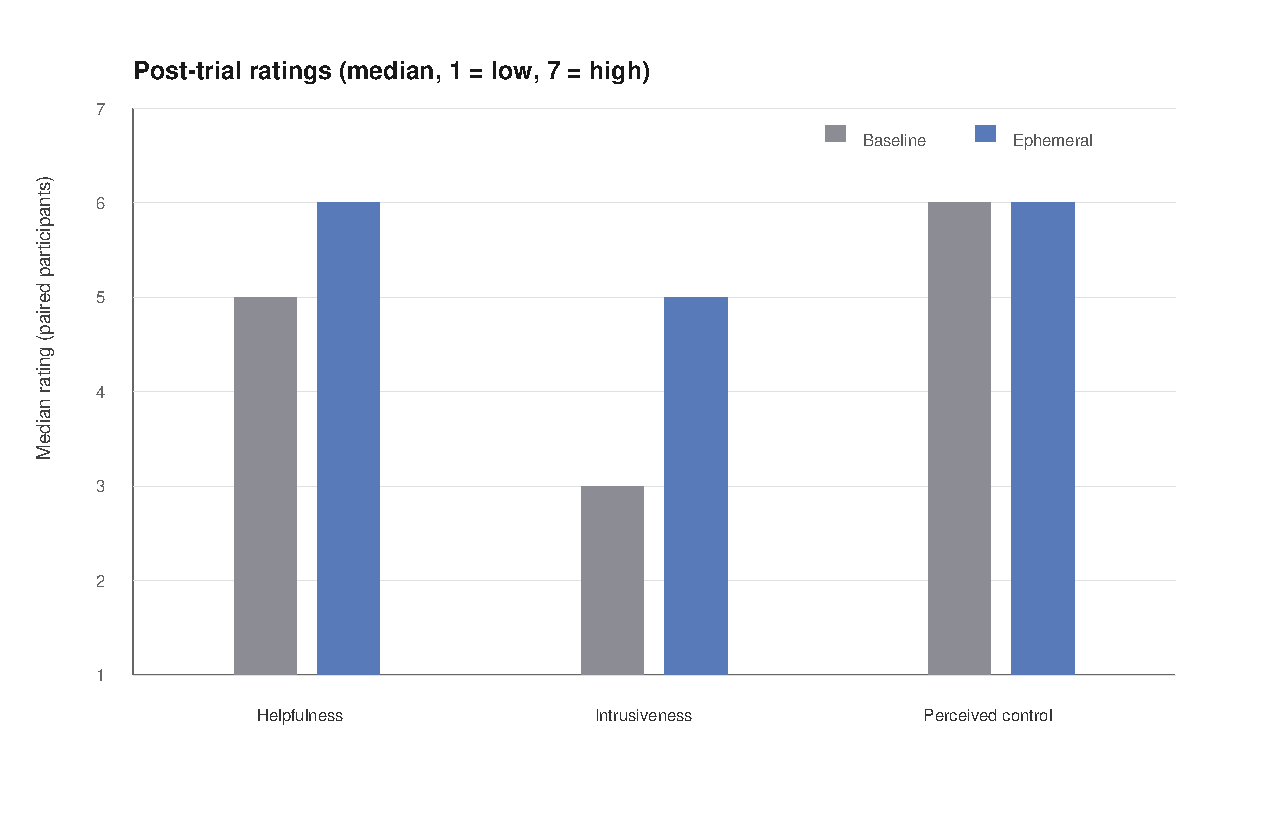
\includegraphics[width=0.75\textwidth]{graphics/results-likert-ratings.pdf}
    \caption{Median post-trial ratings by measure and condition (1 = low, 7 = high). Bars show the median rating across paired participants for each measure.}
    \label{fig:likert}
\end{figure}

\subsection{Overall Preference}

% SQL — final preference (raw A/B/same responses):
% SELECT qr.question_key, qr.response_value, count(*) AS n
% FROM questionnaire_responses qr
% JOIN ( <valid participants subquery> ) v ON v.id = qr.participant_id
% WHERE qr.trial_id IS NULL
%   AND qr.question_key IN ('final_preference', 'final_helpfulness',
%                           'final_intrusiveness', 'final_real_life')
% GROUP BY qr.question_key, qr.response_value
% ORDER BY qr.question_key, qr.response_value;
%
% SQL — final preference mapped to actual condition:
% SELECT
%   qr.question_key,
%   CASE
%     WHEN qr.response_value = 'same' THEN 'no_preference'
%     WHEN (qr.response_value = 'A' AND p.baseline_is_version_a)
%       OR (qr.response_value = 'B' AND NOT p.baseline_is_version_a)
%       THEN 'baseline'
%     ELSE 'ephemeral'
%   END AS actual_preference,
%   count(*) AS n
% FROM questionnaire_responses qr
% JOIN participants p ON p.id = qr.participant_id
% JOIN ( <valid participants subquery> ) v ON v.id = qr.participant_id
% WHERE qr.trial_id IS NULL
%   AND qr.question_key IN ('final_preference', 'final_helpfulness',
%                           'final_intrusiveness', 'final_real_life')
% GROUP BY qr.question_key, actual_preference
% ORDER BY qr.question_key, actual_preference;

After completing both trials, participants answered four forced-choice comparison questions. Responses were stored as Version~A or Version~B and mapped back to the actual experimental condition using each participant's counterbalancing assignment. Table~\ref{tab:preference} summarises the results.

\begin{table}[htbp]
    \centering
    \caption{Final comparative preference questions ($n = \GenNValid$).}
    \label{tab:preference}
    \begin{tabular}{@{}lccc@{}}
        \toprule
        Question & Baseline & Ephemeral & No preference \\
        \midrule
        Overall preference & \GenPrefOverallB{} & \GenPrefOverallE{} & \GenPrefOverallN{} \\
        More helpful & \GenPrefHelpB{} & \GenPrefHelpE{} & \GenPrefHelpN{} \\
        More intrusive & \GenPrefIntrB{} & \GenPrefIntrE{} & \GenPrefIntrN{} \\
        Real-life preference & \GenPrefLifeB{} & \GenPrefLifeE{} & \GenPrefLifeN{} \\
        \bottomrule
    \end{tabular}
\end{table}

\thesistodo{Run a binomial test for the overall preference question excluding no-preference responses, then report whether participants meaningfully favoured one condition.}

\subsection{Ephemeral Support Engagement}

% SQL — ephemeral-only support engagement summary:
% SELECT
%   count(DISTINCT te.trial_id) FILTER (WHERE te.event_type = 'support_triggered') AS trials_triggered,
%   count(DISTINCT te.trial_id) FILTER (WHERE te.event_type = 'support_requested') AS trials_requested,
%   count(DISTINCT te.trial_id) FILTER (WHERE te.event_type = 'support_shown') AS trials_shown,
%   count(DISTINCT te.trial_id) FILTER (WHERE te.event_type = 'support_used') AS trials_used,
%   count(DISTINCT te.trial_id) FILTER (WHERE te.event_type = 'support_dismissed') AS trials_dismissed,
%   count(DISTINCT te.trial_id) FILTER (WHERE te.event_type = 'support_ignored') AS trials_ignored,
%   count(DISTINCT te.trial_id) FILTER (WHERE te.event_type = 'support_inspect_expanded') AS trials_expanded
% FROM trial_events te
% JOIN trials t ON t.id = te.trial_id AND t.condition = 'ephemeral'
% JOIN ( <valid participants subquery> ) v ON v.id = te.participant_id;
%
% SQL — per-participant support event counts:
% SELECT
%   te.participant_id,
%   te.event_type,
%   count(*) AS event_count
% FROM trial_events te
% JOIN trials t ON t.id = te.trial_id AND t.condition = 'ephemeral'
% JOIN ( <valid participants subquery> ) v ON v.id = te.participant_id
% WHERE te.event_type IN ('support_triggered', 'support_requested',
%                         'support_shown', 'support_used',
%                         'support_dismissed', 'support_ignored',
%                         'support_inspect_expanded')
% GROUP BY te.participant_id, te.event_type
% ORDER BY te.participant_id, te.event_type;
%
% SQL — fallback rate:
% SELECT
%   count(*) AS total_generations,
%   count(*) FILTER (WHERE (output->>'usedFallback')::boolean = true) AS fallback_count,
%   round(100.0 * count(*) FILTER (WHERE (output->>'usedFallback')::boolean = true)
%         / count(*), 1) AS fallback_pct
% FROM support_outputs so
% JOIN trials t ON t.id = so.trial_id
% JOIN ( <valid participants subquery> ) v ON v.id = t.participant_id;

To interpret the behavioural and subjective results in context, this subsection reports how participants actually interacted with the ephemeral support layer. These measures apply only to the ephemeral condition.

Of the \GenNValid{} participants who completed the ephemeral trial, support was triggered or explicitly requested in \GenEngNTriggered{} cases (\GenEngPctTriggered{}\%). Once shown, support was actively used (applied or confirmed) in \GenEngNUsed{} cases, dismissed without use in \GenEngNDismissed{} cases, and ignored entirely in \GenEngNIgnored{} cases. \GenEngNExpanded{} participants expanded the support for further detail. The support generation pipeline produced \GenEngTotalGen{} specifications in total, of which \GenEngFallbackCount{} (\GenEngFallbackPct{}\%) fell back to the deterministic fallback because the generated output failed validation.

\thesistodo{Interpret the engagement pattern. If most participants used the support, say the main results are directly interpretable. If many dismissed or ignored it, note that the measured effects may either understate the potential of ephemeral assistance or indicate that the support was not perceived as useful.}

\subsection{Summary of Findings}

\thesistodo{Write a short factual summary of the findings in 4 to 6 sentences. Cover completion rate, completion time, interaction count, subjective ratings, preference, and engagement, and use it as a bridge into the discussion.}

Table~\ref{tab:results-summary} provides an overview of all primary outcome measures.

\begin{table}[htbp]
    \centering
    \caption{Summary of primary outcome measures across conditions.}
    \label{tab:results-summary}
    \begin{tabular}{@{}llll@{}}
        \toprule
        Measure & Baseline & Ephemeral & $p$ \\
        \midrule
        Completion rate & \GenSumCompPctB{}\% & \GenSumCompPctE{}\% & \GenSumMcNemarP{} \\
        Completion time (Mdn, s) & \GenSumTimeBMdn{} & \GenSumTimeEMdn{} & \GenSumTimeP{} \\
        Interaction count (Mdn) & \GenSumIntBMdn{} & \GenSumIntEMdn{} & \GenSumIntP{} \\
        Helpfulness (Mdn) & \GenSumHelpBMdn{} & \GenSumHelpEMdn{} & \GenSumHelpP{} \\
        Intrusiveness (Mdn) & \GenSumIntrBMdn{} & \GenSumIntrEMdn{} & \GenSumIntrP{} \\
        Perceived control (Mdn) & \GenSumCtrlBMdn{} & \GenSumCtrlEMdn{} & \GenSumCtrlP{} \\
        Overall preference & \multicolumn{2}{c}{\GenSumPrefOverall{}} & \GenSumPrefOverallP{} \\
        \bottomrule
    \end{tabular}
\end{table}
